\section{Data Streaming}
Specializing the core computation part of a processor and relying only on traditional memory abstractions is not sufficient for the necessary improvements on modern-day CPUs \cite{8192490}. As a matter of fact an area where specialization has not advanced at the same pace as other components is memory primitives. Exposure to more memory information at the ISA level and utilizing unique micro-architecture mechanics would allow for tackling multiple shortcomings with memory use in the core. Some of these shortcomings are the added overhead in the pipeline on data indexing and memory address generation, the overlapping memory requests, and transfers from the memory system.

The solution for some of these problems might lie in using dedicated structures of memory access such as data streams \cite{8192490}. Data streams are easily constructed through the analysis of repeated patterns of memory accesses, most of the time associated with loops and nested loops of programs.

The following subsections present a brief overview of some recent state-of-the-art proposals to address data streaming in accelerators and general purpose processors.


\subsection{Stream Accelerators for Data Manipulation}
\label{label:stream_dataflow}
Stream Dataflow denotes an implementation of an accelerator proposed by Nowatzki \textit{et al.} \cite{8192490} with the sole purpose of managing streamed memory accesses. According to its authors, the proposed architecture can serve as the basis of configurable memory accelerators.

The acceleration unit proposed in this project was designed with the objective of achieving as good of performance as an application or domain-specific system while trying to maintain efficiency and utilization abstraction. The approach taken to achieve such goals was through the use of data stream memory structures.

\begin{figure}[H]
	\begin{center}
 		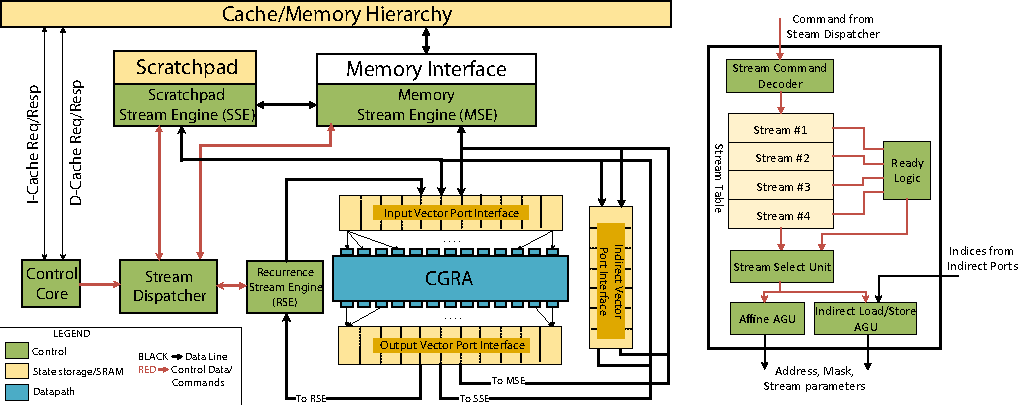
\includegraphics[width=0.87\linewidth]{images/stream-dataflow arch.pdf}
 		\caption{Stream Data Flow micro-architecture (Softbrain) (left); Stream engine pipeline (right) - Figure from \cite{8192490}}
 		\label{fig:stream-dataflow_arch}
	\end{center} 
\end{figure}

The proposed micro-architecture, called \textit{Softbrain}, can be seen in Figure \ref{fig:stream-dataflow_arch} (Left), and it is composed of five primary components:

\begin{itemize}
    \item \textbf{Control Core} - Tasked with the generation of stream-dataflow commands;
    \item \textbf{Stream Dispatcher} - Unit that tracks stream resource dependencies, issues commands to stream engines, and manages concurrent stream execution.
    \item \textbf{Stream Engines} - 3 engines that carry out the data access: one for memory (facilitating wide access to memory), one for scratchpad (efficient data reuse), and one for DFG recurrences (for immediate reuse). The use of each engine is dependent on the streams that are assigned to them.
    \item \textbf{Vector Ports} - The main interface between the computation that is carried out in the CGRA and the streams. A set of isolated vector ports allows for indirect memory loads/stores.
    \item \textbf{Main Acceleration Unit (CGRA)} - The coarse grained reconfigurable pipeline where the main processing of the dataflow graphs is conducted. 
\end{itemize}

The Stream-Dataflow accelerator operates by executing precompiled graphs known as DataFlow Graphs (DFG). The compilation of these graphs occurs alongside program compilation and consists of multiple instructions organized in a network of operations and dependencies. 


During runtime, the main acceleration unit is reconfigured according to the DFG to correctly map the input and output of the vector ports and define the appropriate vector length for compatibility with the memory streams. Additionally, this functional unit is set up for the operations specified by the flow of the graph, creating the advantage of smooth execution of the operations without the need for control inside the CGRA unit.


\subsubsection{Streams}

The stream data structures utilized in the Dataflow Graph Accelerator are defined by 3 parameters: a source location, a destination, and an access pattern. Both the source and destination are associated with a memory address, programmable scratchpads, or a named vector port.

Port locations are associated with the CGRA unit, making the associated streams serve as inputs and outputs of the DFG. 

DFG ports support simple first-in-first-out patterns, while memory and scratchpad access patterns can be more intricate, incorporating features such as strides, repetitions, indirect access, scatter-gather, etc.

Streams typically operate concurrently, but those associated with the same DFG port must execute sequentially.


\subsubsection{Streaming Engines}
In order to be able to utilize stream data structures and take advantage of the high parallelism and low power overheads \cite{8192490}, streaming engines need to be implemented into the micro-architecture. The proposed design for each of the two implemented engines is driven from the diagram illustrated in Figure \ref{fig:stream-dataflow_arch} (Right) and works as a pipeline system.


The engine operates by decoding instructions issued by the dispatcher, keeping track of the number of active streams, and maintaining associated data for each stream. On each clock cycle, the engine selects one of the active streams and generates the required address and data transfer commands. Additionally, it monitors backpressure signals to ascertain if a stream is considered ready. This readiness condition implies that the destination port is not full, and data can be fetched from the source.

As was referred before, the memory system comprises two engines: the memory stream and the scratchpad stream. The memory stream engine is tasked with facilitating the transfer of data to and from the primary memory cache, utilizing streams, and incorporating memory buffering. On the other hand, the scratchpad stream engine bears resemblance to the memory stream engine. However, it is distinct in that it features its dedicated ported SRAM, supporting single-read and single-write operations. 


\subsubsection{Stream-Dataflow ISA}
For the correct operation of the stream-dataflow micro-architecture, three main types of instructions were defined:
\begin{itemize}
    \item[] \Tbullet{T1}{DFG Specification} Given that the physical architecture may impose limitations on the number of instructions for each type in a graph, several constraints on the size of the input and output vectors, and the number of inputs and outputs, the configuration of such parameters could become cumbersome. For that reason, Nowatzki \textit{et al.} \cite{8192490} have chosen to simplify the matter by introducing a single instruction that loads a compiled configuration directly from memory.
    
    \item[] \Tbullet{T2}{Stream Specification} The provided instructions enable the configuration of streams for access with various patterns. These instructions are versatile and can be set up for the most common type of memory access pattern, namely, two-dimensional affine accesses. The definition of such patterns involves specifying the access size, the stride value (size between consecutive accesses), and the number of strides. Additionally, indirect streams can be configured by designating one stream's output as input for another stream.
    
    \item[] \Tbullet{T3}{Barrier Specification} The proposed \acrfull{ISA} includes three barrier instructions. Two of them synchronize the reading and writing of the scratchpad memory, while the third ensures the completion of the \acrfull{DFG} and guarantees that the correct data is stored in the host memory.
\end{itemize}

\subsubsection{Result Analysys}

To assess the goal of designing an accelerator that could replace a domain-specific implementation while maintaining generality, Nowatzki \textit{et al.} \cite{8192490} conducted a series of workload tests from the MachSuite. Each test was run by a \textit{Softbrain} implementation, configured to a max of 20 DFG instructions, and a customized Aladdin ASIC with its implementation generated for each application. %The choosing of the ASIC Design for each test was done through the analysis of multiple implementations in order to find the one closest to the \textit{Softbrain} performance while minimizing power, area, and execution time.
The comparison focused on their power consumption, performance, energy efficiency, and area.

Both the Softbrain and the ASIC implementations showed 1-7x speedup gains across all workloads when compared with a SandyBridge OOO Quad-Core, keeping on par with one another. In terms of power and energy efficiency, the \textit{Softbrain} accelerator showed worse results than the ASICs implementations, however not far behind it. 

On area comparison, the \textit{Softbrain} showed a bigger area use however, since \textit{Softbrain} is programmable on runtime and able to run all workloads, it is possible to advocate that the \textit{Softbrain} implementation is more area efficient than the ASIC implementation since designing a system for the full set of benchmarks performed would require 2.4x the area of \textit{Softbrain}.

Nowatzki \textit{et al.} \cite{8192490} conclude by stating that the developed work demonstrates the potential of designing programmable/configurable architecture that leverage the advantages of streaming structures.


\subsection{Stream-based Memory Access Specialization for General Purpose Processors}

In a follow-up research to the work developed by Nowatzki \textit{et al.} in Stream-Dataflow Acceleration\cite{8192490}, Wang and Nowatzki (2019) \cite{8980305} set out to apply some other same streaming principles on General Purpose Out-of-Order Processors, with the main objective of enhancing the data fetching capabilities of such systems.

Through the use of stream-decoupling, prefetching, and specialized cache policies, the authors aim to reduce the instruction pressure on the processor's pipeline while also making the delivery of data to the processor faster.

\subsubsection{Microachiteture Extension}
In order to keep modifications to the existing microarchitecture to a minimum, most of the frontend structure of the core was maintained unaltered, with the exception of the addition of an iteration map, that tracks the position of each stream index by mapping it to a counter table, the introduction of FIFOs that store the accessed data of the streams, and the implementation of a streaming engine. The location of these units is shown on the left side of Figure \ref{fig:SD_architeture}.

\begin{figure}[H]
\begin{center}
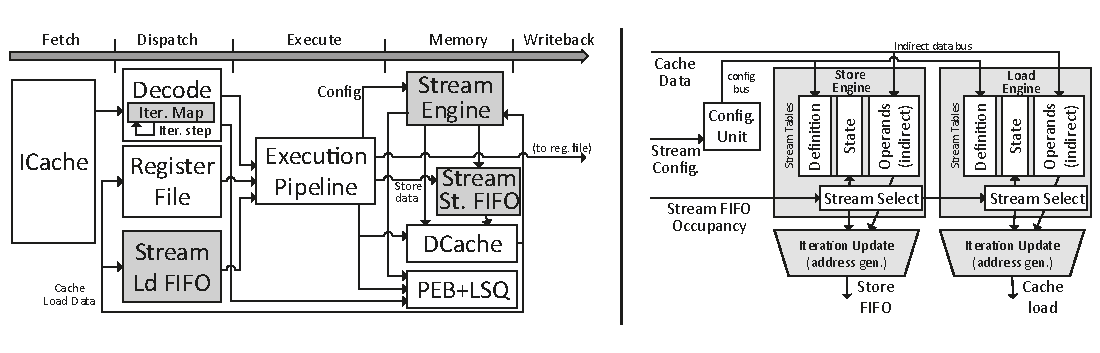
\includegraphics[width=0.87\linewidth]{images/SD_architeture.pdf}
\caption{Stream Specialized Pipeline (Left); Stream Engine (Right) - Figure adapted from \cite{8980305}}
\label{fig:SD_architeture}
\end{center}
\end{figure}


The streaming engine comprises two identical units, one designated for loading from memory and the other for storing in memory. These units incorporate a set of tables employed to describe the state of any configured stream. The \textbf{definition table }encompasses the pattern (affine, indirect, linked) along with the parameters of the access (stride, width, size). The second table is the \textbf{state table }, responsible for storing the memory view of the induction variables, indicating the current address. Lastly, the \textbf{operands table }contains information on any stream dependencies.
Through the use of this stored information, the streaming engine generates, on each clock cycle, the memory address of the following reads/stores caused by the execution pipeline.

The FIFOs of the streaming engine have the purpose of holding the decoupled state either for storing or loading. Whenever a core instruction makes a read to a stream, it accesses the data on the load FIFO. Whenever a core instruction performs a store, the value to store is combined with a previously generated address kept in the store FIFO.


\subsubsection{Decoupled-Stream ISA}

The stream-specialized interface proposed by Wang and Nowatzki (2019) \cite{8980305}, tries to maintain the stream data structure implementation separated from the rest of the cores' microarchitecture maintaining a higher level of abstraction. This is made through the use of special pseudo-registers to which the execution pipeline has access and are mapped to specific data streams. The streaming part of the system applies a similar principle to the Stream Dataflow Accelerator in the sense that it is configurable through an initial instruction.

The execution of code compiled for this stream interface contains such instruction at the beginning of code sections that will benefit from data streaming (loop portions of code). It is responsible for: \textbf{setting up} the necessary \textbf{pseudo-registers} employed by the core pipeline and mapped to the \textbf{data streams}, configuring the \textbf{streams type} (induction/memory) and \textbf{pattern} (stride, width, and optional length),  the dependencies and the starting address. The configuration of streams can also be made to address another stream, thereby establishing a dependency through indirect memory access.

During the execution of the code in the pipeline, a "step" instruction is employed to advance the position of the stream by modifying the induction variables related to the streams and providing the core with abstract information on the stream's progress. At the end of the loop iterations, the configured streams are deallocated and released for the next utilization.

The proposed Instruction Set Architecture (\acrshort{ISA}) incorporates a set of instructions that enable fundamental stream operations, like pattern definitions and data width configuration, supporting complex accesses to data and coalescing of data structures. 

Figure \ref{fig:SD_execution} depicts four examples of the decoupled-stream pseudo-code, along with its stream dependence graph.

\begin{figure}[H]
\begin{center}
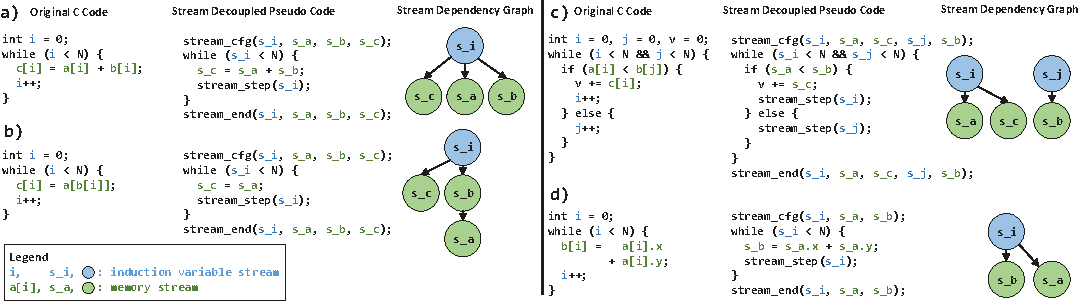
\includegraphics[width=0.97\linewidth]{images/SD_execution.pdf}
\caption{Pseudo Code Examples - Figure adapted from \cite{8980305}}
\label{fig:SD_execution}
\end{center}
\end{figure}

\textbf{\textit{stream\_cfg}} is the instruction used for the configuration, defining all the streams within the loop. After configuration, the stream engine can start fetching data based on the knowledge previously defined.

The use of \textbf{\textit{stream\_step}} inside loop iterations advance the induction variable stream, altering the stream pseudo-register position and resulting in a cascade on all dependent streams. This behavior is evident in the Stream Dependency Graph, where the advancement of \textit{s\_i} causes all dependent streams (\textit{s\_a, s\_b, s\_c, ...}) also to advance.

The \textbf{\textit{stream\_end}} instruction, as the name implies, the utilization of streams concludes by deallocating and releasing the mapped pseudo-registers.

The proposed \acrshort{ISA} comes with its limitations since the decoupling nature of the implementations becomes limited whenever the access patterns cannot be determined at the configuration step. Such cases are conditionally used data and unknown length for an access pattern.


\subsubsection{Using Stream Information}
Wang and Nowatzki (2019) \cite{8980305} also propose the exploitation of the stream information provided by the decoupled design of the presented implementation. Accordingly a prefetching technique and stream-aware cache bypass policies were implemented leveraging such stream information.

In what concerns the prefetching, the distance in which prefetching is made can highly impact the smooth operation of a cores' pipeline. In an ideal prefetcher, the required data would be provided whenever the corresponding load instruction is ready to be issued. This means that a sign of poor performance of the prefetcher could be falling behind on the data requests. For the monitoring and correct utilization of the resources of the processor, Wang and Nowatzki (2019) \cite{8980305} took the approach of implementing a set of counters that track the number of stalls that occur with each stream pseudo-register, entitling it as the dynamic throttling prefetching system. These counters enable the pipeline to dynamically readjust the size distribution of the Load FIFO across stream pseudo-registers. This adjustment provides streams with increased available space and subsequently allow the prefetching distance of specific streams to be incremented based on the rate at which data is being consumed.

In the proposed implementation, the initial value of each stream pseudo-register length is defined in the configuration step with a default value. However, this could be further improved by defining a more personalized value during compilation.

Another technique implemented by Wang and Nowatzki (2019) \cite{8980305} that leverages the information given by the patterns defined by streams, is cache bypassing. In memory requests with low temporal locality, the utilization of cache can become a problem and hurt the overall execution performance. Through the stream information provided by the system (memory footprint, stream length, reuse distance etc), it is possible to decide whether a memory request should be made to the cache or bypass it completely and request the information directly to the memory system. This technique would help avoid polluting the cache with data that would not be reused, as well as avoid unnecessary time wasted with tag lookup and MSHR allocation.


\subsubsection{Result Analysis}

Wang and Nowatzki (2019) \cite{8980305} concluded through a series of workloads that their proposed decoupled-stream ISA extension show very promising results in terms of performance and energy consumption when compared with the baseline simulated 8-Way OOO processor. The tests conducted were made to evaluate the impact of the improvements suggested by the authors, like the inclusion of streaming with prefetching, the utilization of a dynamic throttle of the prefetching distance, and the utilization of stream access information in cache bypassing policies.

The implementation of just the streaming engine resulted in an overall gain of 1.20x in performance. Utilizing both the dynamic throttle (prefetching stall counters) and stream-aware cache policies pushed the gain value to 1.67x when compared with the baseline out-of-order core. In terms of energy efficiency, the implementation of the proposed full system resulted in an improvement of 1.53x compared to the baseline.

Wang and Nowatzki (2019) \cite{8980305} concluded that utilizing the benefits of stream-based prefetching, address computation decoupling, and stream-aware cache policies can lead to a faster, more specialized access and communication within the cache and memory hierarchy, albeit with certain limitations like the problem of unknown length of patterns during stream configuration.

Some further research topics like vector data manipulation could also be seen as a possible improvement to the described system leveraging parallel computation of data.

\subsection{Stream Semantic Registers}
\label{label:ssr}

Stream Semantic Registers (SSR) \cite{9068465} introduces an innovative approach to address the von Neumann bottleneck in single-issue processor cores. This bottleneck arises from the explicit fetch and issue of load/store instructions for data to reach the Arithmetic Logic Units (ALUs) and Functional Units (FUs). In order to mitigate this bottleneck, Schuiki \textit{et al.} \cite{9068465} presents a solution in the form of a straightforward and lightweight RISC-V ISA extension. This extension implicitly encodes memory accesses, thereby reducing the number of instructions associated with memory accesses and enhancing the overall energy efficiency of the system.

To enable this capability, SSR gives some registers stream semantics, meaning that reading from or writing to such registers triggers a direct read or write operation in the memory. This innovative approach streamlines the execution of instructions and contributes to energy efficiency.

\subsubsection{Micro-achiteture}

The following modifications to the processor's core are necessary to implement the SSR system, and allow the mapping of register access to the stream interfaces:

\begin{itemize}
\item[] \Tbullet{C1}{Register File Extension:} Expanding the register file to facilitate the interception and rerouting of accesses to a subset of registers.
\item[] \Tbullet{C2}{Stream Interfaces:} Incorporating stream interfaces to each register file port to allow stream semantics registers.
\item[] \Tbullet{C3}{Control:} Implementing a Control and Status Registers (CSR) to enable or disable stream semantics.
\item[] \Tbullet{C4}{Data Paths:} Adding the paths needed for the communication of stall conditions and back-pressure path to the core's main controller.
\end{itemize}

Schuiki \textit{et al.} \cite{9068465} designed the needed modifications with the added intent of minimizing the impact on the complexity of the underlying architecture. A high-level schematic of the architectural changes needed for this implementation can be seen in Figure. \ref{fig:ssr-overview}.

\begin{figure}[H]
	\begin{center}
 		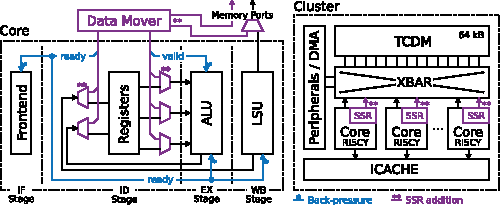
\includegraphics[width=0.87\linewidth]{images/ssr-overview.pdf}
 		\caption{High-level data flow of the SSR extension in a single core  - Figure from \cite{9068465}}
 		\label{fig:ssr-overview}
	\end{center} 
\end{figure}

\subsubsection{Register Files}

The primary architectural modification introduced by the SSR extension is in the processor register file. This register file is structured as a default three read and two write port configuration. However, each port is customized to incorporate the needed circuitry (refer to Fig. \ref{fig:ssr-stream_enable_check}) to intercept read/write accesses and detect whether the specified register has stream semantics enabled.

The process of a register access unfolds as follows: the access is intercepted, the presence of stream semantics is determined, and if confirmed, the access is rerouted to the respective external stream interface connected to the data mover unit.

\begin{figure}[H]
	\begin{center}
 		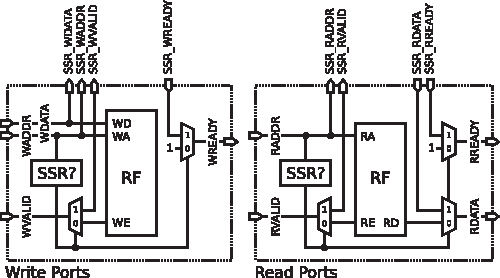
\includegraphics[width=0.67\linewidth]{images/ssr-circuitry.pdf}
 		\caption{Required circuits for stream semantic enabled verification  - Figure from \cite{9068465}}
 		\label{fig:ssr-stream_enable_check}
	\end{center} 
\end{figure}

The confirmation of the active status of stream semantics is carried out in the \textit{SSR} section of the circuit, as illustrated in Fig. \ref{fig:ssr-stream_enable_check}. This verification involves checking the following conditions:

\begin{itemize}
\item[1] The register address connected to the WADDR or the RADDR must correspond to one of the registers allowed to utilize stream semantics, on the write ports circuit or read ports circuit, respectively;
\item[2] The stream semantics flag must be enabled in the core's CSR;
\end{itemize}

In case both conditions are true then the transaction is routed out of the core through a stream interface to the data mover.

\subsubsection{Data Mover}

The accesses initiated within the core and directed outward through the stream interfaces reach the data mover unit. This segment of the architecture, visible in Figure \ref{fig:ssr-data_mover} is tasked with accurately mapping the incoming accesses to the memory system. To execute this function, the data mover incorporates a set of lanes, each comprising a \textit{First-In-First-Out (FIFO)} queue buffer and an address generator unit (AGU). The AGU is responsible for associating each streamed access with the corresponding memory address, whether for reading or writing. Offloading the memory address generation outside of the main pipeline reduces the pressure caused by this type of function.

The internal diagram of the AGU can be seen on the right of Figure \ref{fig:ssr-data_mover} and is based on AGU presented by Schuiki \textit{et al.} \cite{8502059}. It works through the configuration of the hardware loops ($L0$ to $L3$), which are composed of 16-bit counters that iterate over the parameters of the stream access pattern and provide the values necessary for the address generation. 

\begin{figure}[H]
	\begin{center}
 		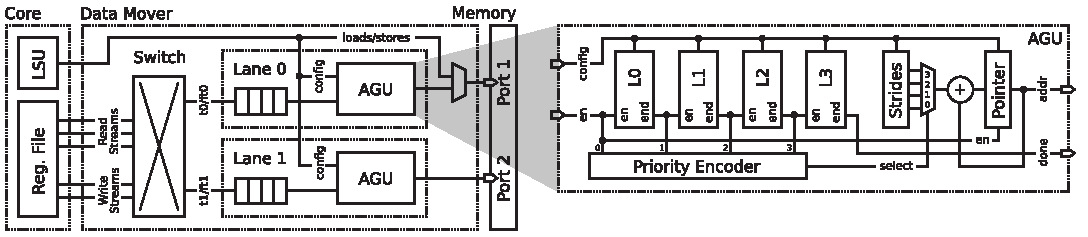
\includegraphics[width=0.87\linewidth]{images/ssr-data_mover.pdf}
 		\caption{Data mover interfaces and inner structure (Left); Internal design of Address Generator Unit (Right) - Figure adapted from \cite{9068465}}
 		\label{fig:ssr-data_mover}
	\end{center} 
\end{figure}

For each processed stream, the AGU is configured in either reading mode, generating memory addresses, or writing mode, producing tags for each datum to be written. It's noteworthy that the processing of streams cannot be interleaved; thus, the same mode has to persists per AGU until the conclusion of the address pattern.


A positive aspect arising from the previously mentioned constraint is the proactive capability of the data mover to perform memory reads using the defined configuration. This behavior facilitates quicker access to data, as whenever the processor decides to read from an SSR, the data is already available. This stands in contrast to normal data accesses, where each request needs to be individually made and awaited.

Unfortunately, due to the design of the data mover and the pro-active read, memory incoherence could occur since a lane could have read a value from memory and placed it in the \textit{FIFO} before the other lane could have updated the same memory location with a new value, for this reason, to avoid data races write operation cannot initiate on a section of memory that has been set to read from.

\subsubsection{Execution Flow}

The execution of a program compiled for this solution starts with the setup of the configuration registers present in the AGUs of the data mover. These registers define the loop dimensions of a stream, allowing for a total of four dimension loops. After the activation of stream semantics in the cores' CSR the iteration of the computations occurs with the AGU loop counters iterating over the preconfigured access patterns and providing the necessary data to the main pipeline of the core.

At the end of the code section optimized for the use of stream semantics, the program executes an instruction to deactivate the use of stream semantics, allowing the core to utilize every register as normal registers.

\subsubsection{Result Analysis}


Several tests were conducted with a focus on evaluating power consumption, performance, efficiency, and the implementation area. In their research, Schuiki \textit{et al.} \cite{9068465} observed a performance increase ranging from 2x to 5x, attributed to the overall reduction in instructions. This improvement was achieved with only a minor increase in the core area (11\%), accompanied by a notable decrease in cache energy consumption by up to 5.6x. These findings substantiate the belief in the potential effectiveness of streaming mechanisms.

While the outcomes achieved for the compiled workloads were favorable, there is room for improvement in the compilation method. The current compiler approach applies SSR indiscriminately to every encountered loop, this leads to the utilization of SSR in smaller loops that do not derive significant benefits, mainly due to the higher setup time required. This observation underscores a potential drawback and emphasizes the necessity for additional research and enhancements.

As also highlighted by Schuiki \textit{et al.} \cite{9068465}, the design of the Address Generator Unit (AGU) in the data mover restricts the applicability and gains of the implementation, primarily due to the limitations in the types of memory access patterns that can be configured. Other research has explored similar principles to those used in SSR but with the capability to accommodate more intricate data patterns, like the Indirection Stream Semantic Register (ISSR) extension \cite{9474230}.


